\documentclass[a4paper, 12pt]{extarticle}

%%% Includes 
\usepackage[utf8]{inputenc} % UTF-8 encode 
\usepackage[english, russian]{babel}
\usepackage{geometry} % adjust page layout 
\usepackage{graphicx} 
\usepackage{hyperref} 
\usepackage{amsmath} % math formulas 
\usepackage{setspace} % for set line spacing 
\usepackage{indentfirst} % indent on a first line after the paragraph 
% \usepackage{pgfplots} % for plots 
\usepackage{listings} % for code listings 
\usepackage{xcolor} % colors (used for listings)
\usepackage{sourcecodepro} % for another monospaced font 
\usepackage{cmap} % for correct search in pdf
\usepackage{placeins} % for \FloatBarrier


%%% Debug
% \usepackage{showframe} % frame borders for demonstration 


%%% Custom commands
% commands for unnumbered sections
\newcommand{\usection}[1]{\section*{#1} \addcontentsline{toc}{section}{\protect\numberline{}#1}}
\newcommand{\usubsection}[1]{\subsection*{#1} \addcontentsline{toc}{subsection}{\protect\numberline{}#1}}
\newcommand{\usubsubsection}[1]{\subsubsection*{#1} \addcontentsline{toc}{subsubsection}{\protect\numberline{}#1}}


% Redefinition of section and subsection numbering style (with dot at the end)
\def\thesection{\arabic{section}.}
\def\thesubsection{\arabic{section}.\arabic{subsection}.}
\def\thesubsubsection{\arabic{section}.\arabic{subsection}.\arabic{subsubsection}.}



%%% Settings for links 
\hypersetup{
    colorlinks,
    citecolor=black,
    filecolor=black,
    linkcolor=black,
    urlcolor=blue
}



%%% Layout
\geometry{
	left=17mm, % left margin
	top=17mm, % top margin
	right=17mm, % right margin
	bottom=20mm, % bottom margin
	marginparsep=0mm, % space between text and margin notes
	marginparwidth=0mm, % width of margin notes
	headheight=8mm, % height of the header
	headsep=5mm, % space between header and text
}


\linespread{1.5} % line spacing
\setlength{\parskip}{\baselineskip}  % Add space between paragraphs


% overfull hbox settings
\tolerance 5000 % default 200, max 10000, 
\hbadness 3000 % default 1000, max 10000, warning threshold for underfull hbox
\emergencystretch 0pt  % default 0pt, how much the lines can stretch for the sake of good line breaks
\hfuzz 0.4pt % ignore overfull box less than 
\widowpenalty=10000 % no lines at the start of the page
\vfuzz \hfuzz % don't care about underfull vbox if overfull is acceptable
\raggedbottom % if the page is not filled, align the content to the bottom


%%% Redefinition of table of contents command to get centered heading
\makeatletter
\renewcommand\tableofcontents{ 
  \begin{singlespace}
    \null\hfill\textbf{\Large\contentsname}\hfill\null\par
    \@mkboth{\MakeUppercase\contentsname}{\MakeUppercase\contentsname}%
    \@starttoc{toc}
  \end{singlespace}
}
\makeatother


%%% Listings settings
\definecolor{codegreen}{rgb}{0, 0.6, 0}
\definecolor{codegray}{rgb}{0.5, 0.5, 0.5}
\definecolor{codepurple}{rgb}{0.58, 0, 0.82}
\definecolor{backcolour_gray}{rgb}{0.98, 0.98, 0.98}

\lstdefinestyle{python_white}{
  language=Python,
  backgroundcolor=\color{backcolour_gray},   
  commentstyle=\color{codegreen},
  keywordstyle=\color{blue},
  numberstyle=\tiny\color{codegray},
  stringstyle=\color{codepurple},
  basicstyle=\ttfamily\small\singlespacing,
  breakatwhitespace=true,         
  breaklines=true,                 
  captionpos=b, % t/b                  
  keepspaces=true,                 
  numbers=none, % none/left/rigth                    
  numbersep=5pt,                  
  showspaces=false,                
  showstringspaces=false,
  showtabs=false,                  
  tabsize=2,
  frame=single, % none/leftline/topline/bottomline/lines/single/shadowbox
  rulecolor=\color{gray}, % frame color 
}

\lstset{style=python_white} % set default listings style


% For title page
\def\name{Отчет по лабораторной работе №5} 
\def\subname{<<Преобразование Хафа>>}
\def\madeby{Александр Иванов, Ф ТЕХ.ЗРЕНИЕ 1.1 \\ Ани Аракелян, ТЕХ.ЗРЕНИЕ 1.1\\ Никита Братушка, ТЕХ.ЗРЕНИЕ 1.3}
\def\teacher{Шаветов С. В.}

\begin{document}

% Title page 
\begin{titlepage}

\thispagestyle{empty}

\title{


\includegraphics[width=4cm]{images/ITMO_logo.png} 

\vspace{1em}
НИУ ИТМО 
\vspace{4em}

\begin{center}
\large\textsc{\textbf{\name}}

\vspace{1em}
\subname

\end{center}

\vspace{3em}

\begin{flushright}
\normalsize{ 
Выполнили: \\ \textbf{\madeby} 

Преподаватель: \\ \textbf{\teacher} 
}
\end{flushright}	

\vfill

\begin{center}
\small{Санкт-Петербург, \the\year}
\end{center}
}


\author{}
\date{}
\maketitle
\thispagestyle{empty}
\end{titlepage} % Title page

\addtocounter{page}{1} % Inc counter to start from 2 
\tableofcontents % Table of contents
\pagebreak

\section{Поиск прямых}
\subsection{Исходные изображения}

\subsection{Код на питоне}
\subsection{Результаты поиска}
\subsection{Бонус. Клином красным бей белых!}




\section{Поиск окружностей}
\subsection{Исходные изображения}
Настало время подобрать изображения, содержащие окружности. Мы, авторы этого отчёта --- господа спортивные, поэтому для этого задания мы использовали самый известный символ спортивного движения:

\begin{figure}[ht!]
    \centering
    
\includegraphics[width=0.55\textwidth]{images/circles/source/olympic.jpeg}
    \caption{Олимпийский флаг}
    \label{img:ol_logo}
\end{figure} 

Мы не имели никакого права не обратиться к произведениям основоположника абстракционизма и нашего соотечественника --- Василия Васильевича Кандинского:

\begin{figure}[ht!]
    \centering
    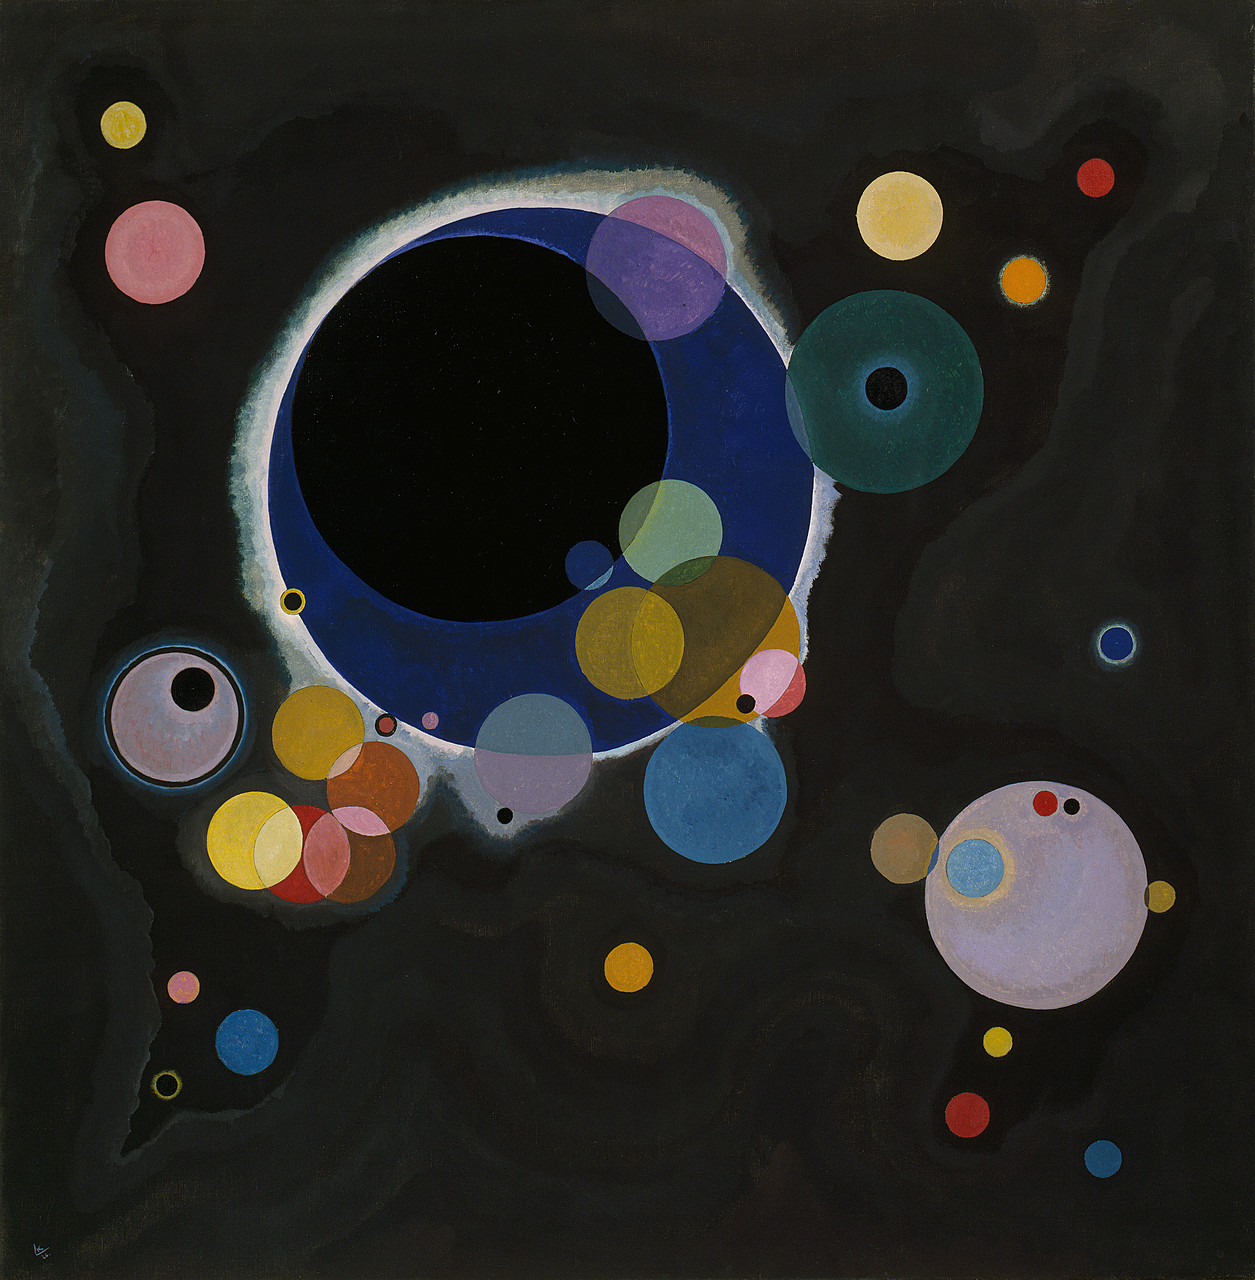
\includegraphics[width=0.55\textwidth]{images/circles/source/Kandinsky_Several_Circles.jpg}
    \caption{В.В. Кандинский -- Несколько кругов}
    \label{img:kan_logo}
\end{figure} 

\clearpage

Последним изображением стала фотография Mercedes-Benz 300 SEL AMG <<Красная свинья>>, ставший ключевым элементом в первом для новой компании AMG триумфе в автогонках:
\begin{figure}[ht!]
    \centering
    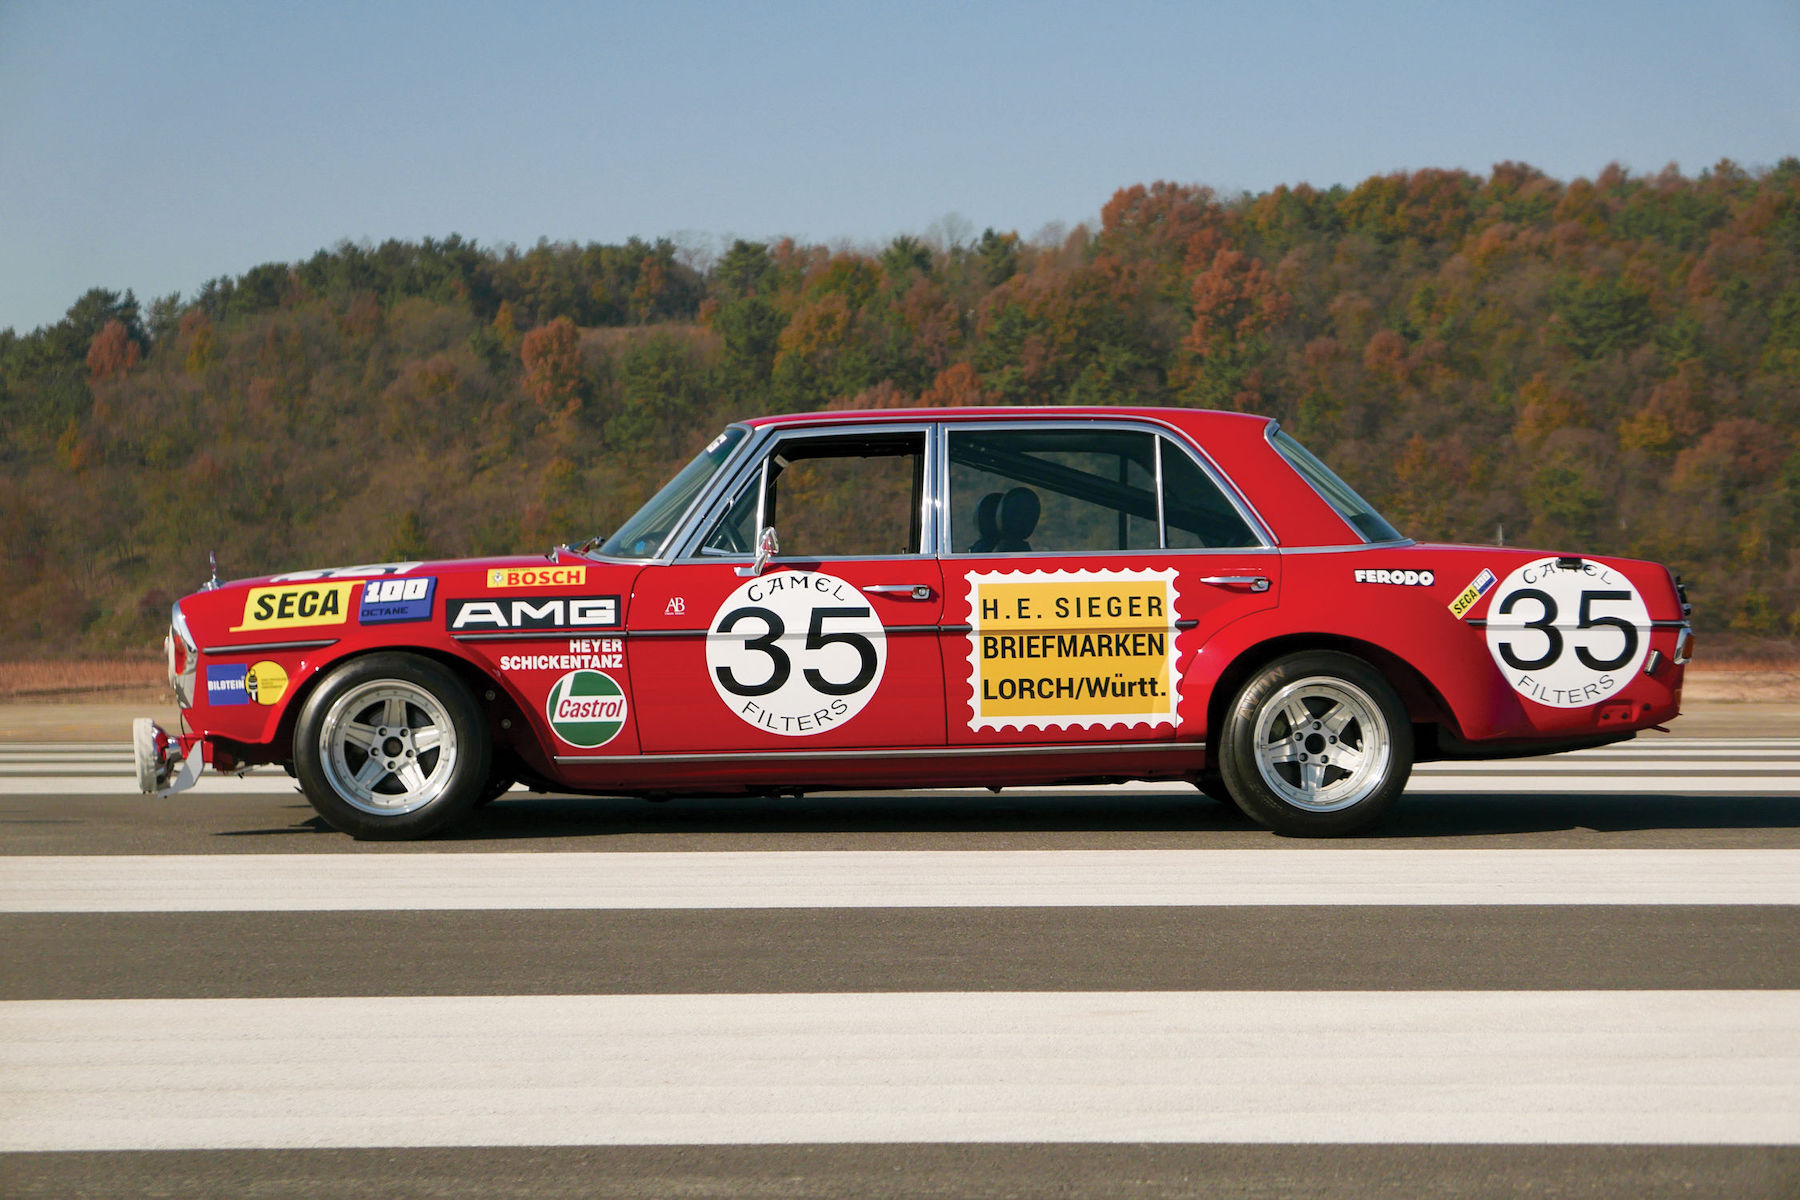
\includegraphics[width=0.55\textwidth]{images/circles/source/Mercedes 300 SEL 6.8 AMG red pig.jpg}
    \caption{ Mercedes-Benz 300 SEL AMG <<Красная свинья>>}
    \label{img:mr_logo}
\end{figure} 

\subsection{Программа на языке Python}
\begin{lstlisting}[caption={Исходный код функции для нахождения и отображения окружностей с помощью преобразования Хафа}, label={lst:line_compute}]
    def circle_detection(option, image):
        # creating image copies
        result = image.copy()
        result_r = image.copy()
        edged = image
        match option:
            case 0:
                # output of the original image
                cv.imshow('Source Image', image)
                cv.waitKey(0)
            case 1:
                # Hough transform
                # Specified radius
                hough_radius = np.arange(180, 181)
                # Getting Hough accumulator
                hough_res = skimage.transform.hough_circle(edged, hough_radius)
                # Getting coordinates for centers of circles 
                ha, cx, cy, radii = skimage.transform.hough_circle_peaks(hough_res, hough_radius, total_num_peaks=1)
                for center_y, center_x, radius in zip(cy, cx, radii):
                    # overlaying circles of specified radius
                    cv.circle(result, (center_x, center_y), int(radius), (255, 255, 0), 10, cv.LINE_AA)
                # Radius range
                hough_radius_r = np.arange(175, 239)
                # Getting Hough accumulator
                hough_res_r = skimage.transform.hough_circle(edged, hough_radius_r)
                # Getting coordinates for centers of circles 
                ha, cx, cy, radii = skimage.transform.hough_circle_peaks(hough_res_r, hough_radius_r, total_num_peaks=4)
                for center_y, center_x, radius in zip(cy, cx, radii):
                    # overlaying circles
                    cv.circle(result_r, (center_x, center_y), int(radius), (255, 255, 0), 10, cv.LINE_AA)
                # transferring recieved images and data to function of creating a comparative image
                image_displaying(image, edged, result, result_r, hough_radius[0], hough_radius_r[0], hough_radius_r[-1])
                # cv.imwrite('results/circles/Mercedes_SP.jpg', result)
                # cv.imwrite('results/circles/Mercedes_R.jpg', result_r)
            case _:
                print('Wrong option! Enter the right number')
    \end{lstlisting}

    \begin{lstlisting}[caption={Исходный код функции для создания сравнительного изображения с результатами преобразования}, label={lst:show_images}]
        def image_displaying(source, canny, finale, finale_r, sp, mn, mx):
            # creating figure with mosaic layout
            fig, axs = plt.subplot_mosaic([['src', 'can'], ['fin', 'finr'], ['info', 'infor']], layout='tight',
                                        figsize=(9.2, 7.8))
            # plotting images
            axs['src'].imshow(cv.cvtColor(source, cv.COLOR_BGR2RGB))
            axs['can'].imshow(canny, cmap=matplotlib.cm.gray)
            axs['fin'].imshow(cv.cvtColor(finale, cv.COLOR_BGR2RGB))
            axs['finr'].imshow(cv.cvtColor(finale_r, cv.COLOR_BGR2RGB))
            # turning off axes
            axs['src'].axis('off')
            axs['can'].axis('off')
            axs['fin'].axis('off')
            axs['finr'].axis('off')
            axs['info'].axis('off')
            axs['infor'].axis('off')
            axs['src'].set_title('Image')
            axs['can'].set_title('Canny edges')
            axs['fin'].set_title('Hough (Specified radius)')
            axs['finr'].set_title(' Hough (Range)')
            # plotting the specified radius size
            axs['info'].text(0.5, 0.5, f'Radius length:{sp}', size=25,
                            ha='center',
                            va='center',
                            bbox=dict(boxstyle="square",
                                    ec=(1., 0.5, 0.5),
                                    fc=(1., 0.8, 0.8)
                                    )
                            )
            # plotting minimum and maximum radius sizes
            axs['infor'].text(0.5, 0.5, f'Min radius: {mn}\nMax line: {mx}', size=25,
                            ha='center',
                            va='center',
                            bbox=dict(boxstyle="square",
                                        ec=(1., 0.5, 0.5),
                                        fc=(1., 0.8, 0.8)
                                        )
                            )
            # displaying and saving the plot
            plt.show()
            fig.savefig('results/circles/olympic.jpg')
            plt.close()
        \end{lstlisting}

\subsection{Результаты преобразования}

\begin{figure}[ht!]
    \centering
    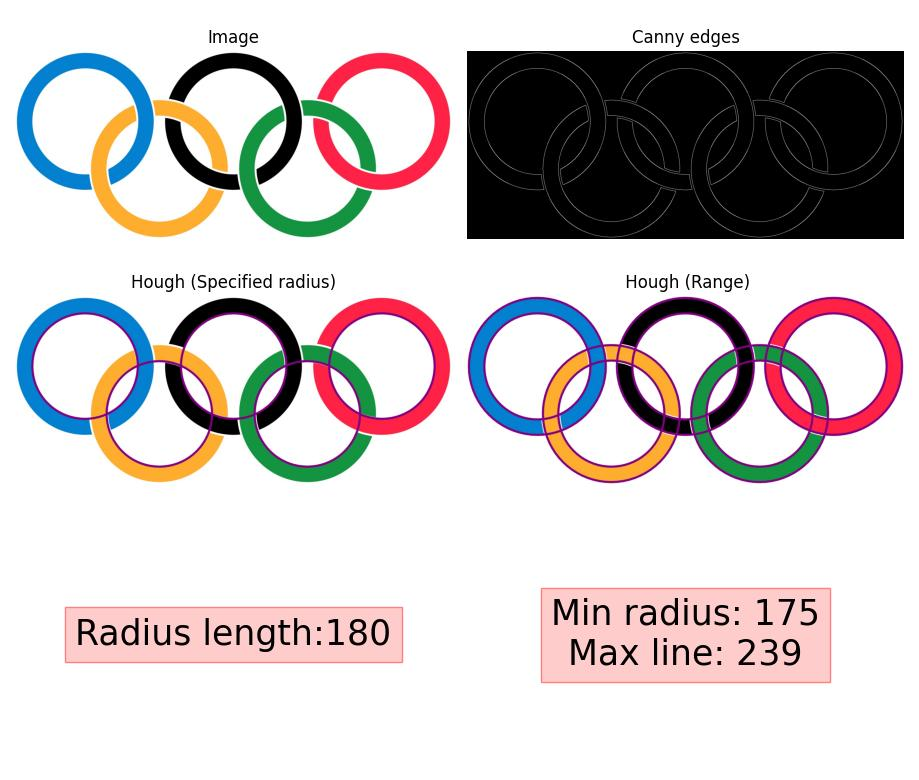
\includegraphics[width=0.8\textwidth]{images/circles/olympics.jpg}
    \caption{Исходное изображение 1; контуры изображения, полученные алгоритмом Кэнни; результаты преобразования Хафа для определенного радиуса и диапазона радиусов}
    \label{img:fin_ol}
\end{figure}

\begin{figure}[ht!]
    \centering
    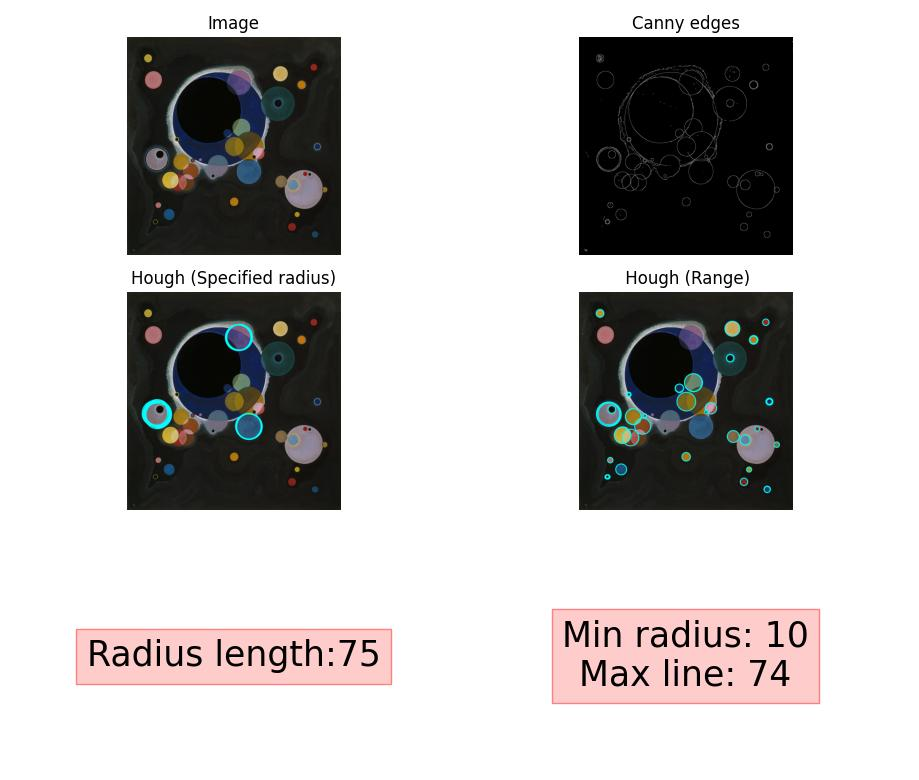
\includegraphics[width=0.8\textwidth]{images/circles/Kandinsky_Several_Circles.jpg}
    \caption{Исходное изображение 2; контуры изображения, полученные алгоритмом Кэнни; результаты преобразования Хафа для определенного радиуса и диапазона радиусов}
    \label{img:kan_fin}
\end{figure}

\begin{figure}
    \centering
    \begin{subfigure}[b]{0.4\textwidth}
        \centering
        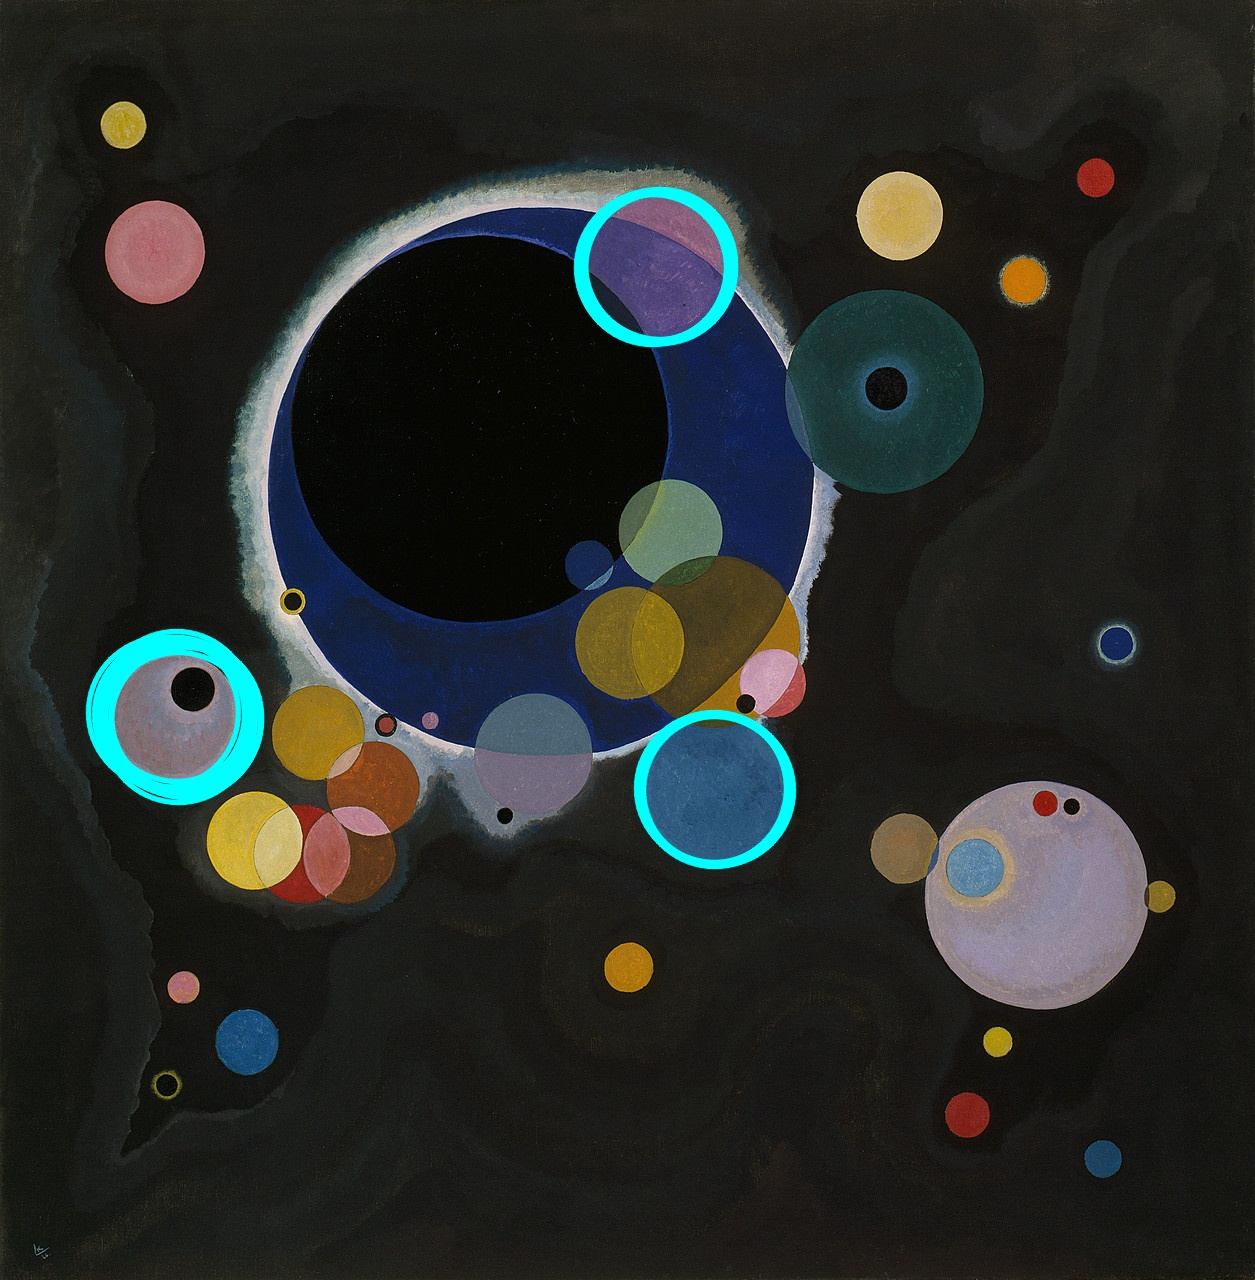
\includegraphics[width=\textwidth]{images/circles/Kandinsky_Several_Circles_SP.jpg}
        \caption{Результат преобразования Хафа для определенного радиуса окружностей}
        \label{img:kan_sp}
    \end{subfigure}
    \hfill
    \begin{subfigure}[b]{0.4\textwidth}
        \centering
        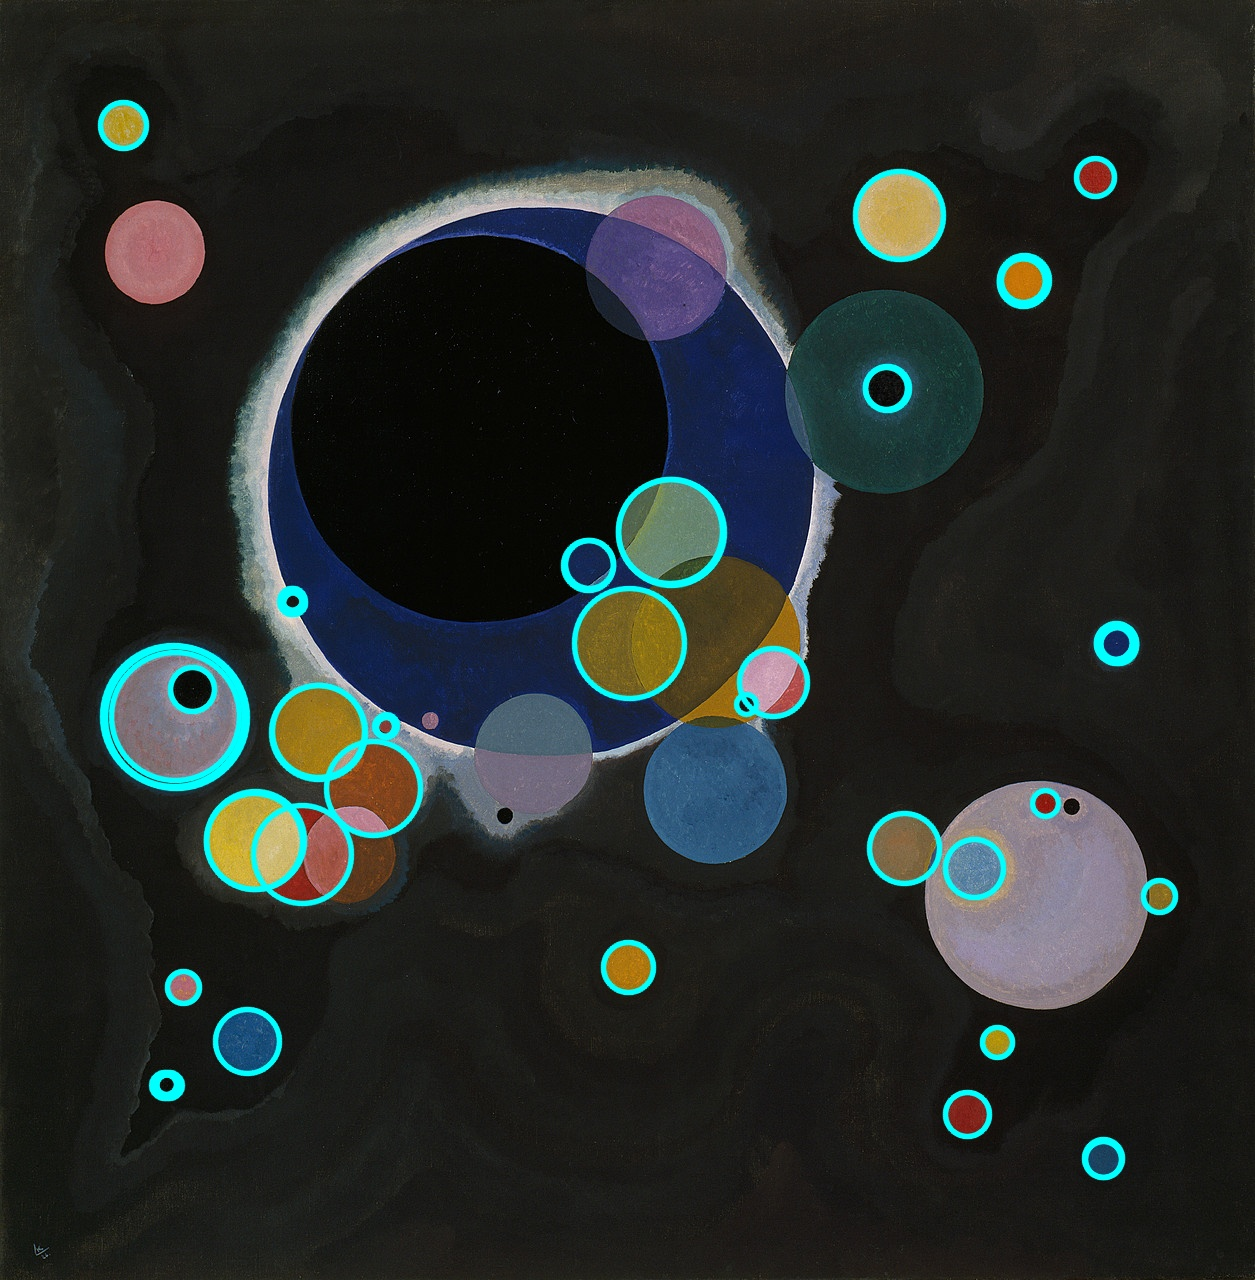
\includegraphics[width=\textwidth]{images/circles/Kandinsky_Several_Circles_R.jpg}
        \caption{Результат преобразования Хафа для диапазона радиусов}
        \label{img:kan_r}
    \end{subfigure}
        \caption{Результаты преобразования Хафа}
       \label{img::kan_comp}
\end{figure}

\begin{figure}[ht!]
    \centering
    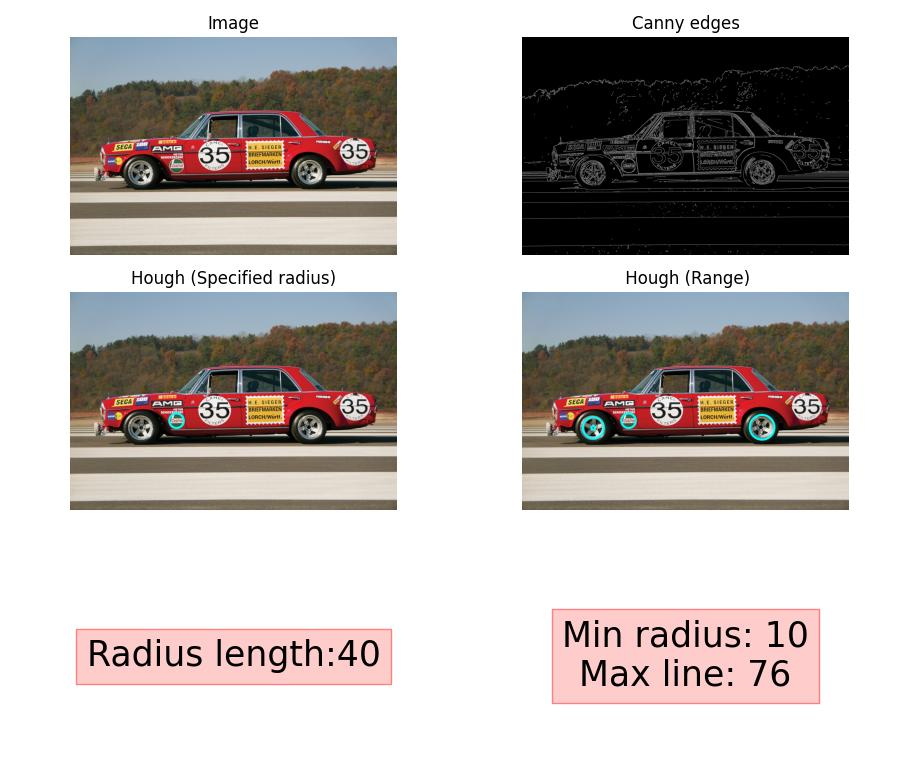
\includegraphics[width=\textwidth]{images/circles/Mercedes.jpg}
    \caption{Исходное изображение 3; контуры изображения, полученные алгоритмом Кэнни; результаты преобразования Хафа для определенного радиуса и диапазона радиусов}
    \label{img:mr_fin}
\end{figure}

\begin{figure}
    \centering
    \begin{subfigure}[b]{\textwidth}
        \centering
        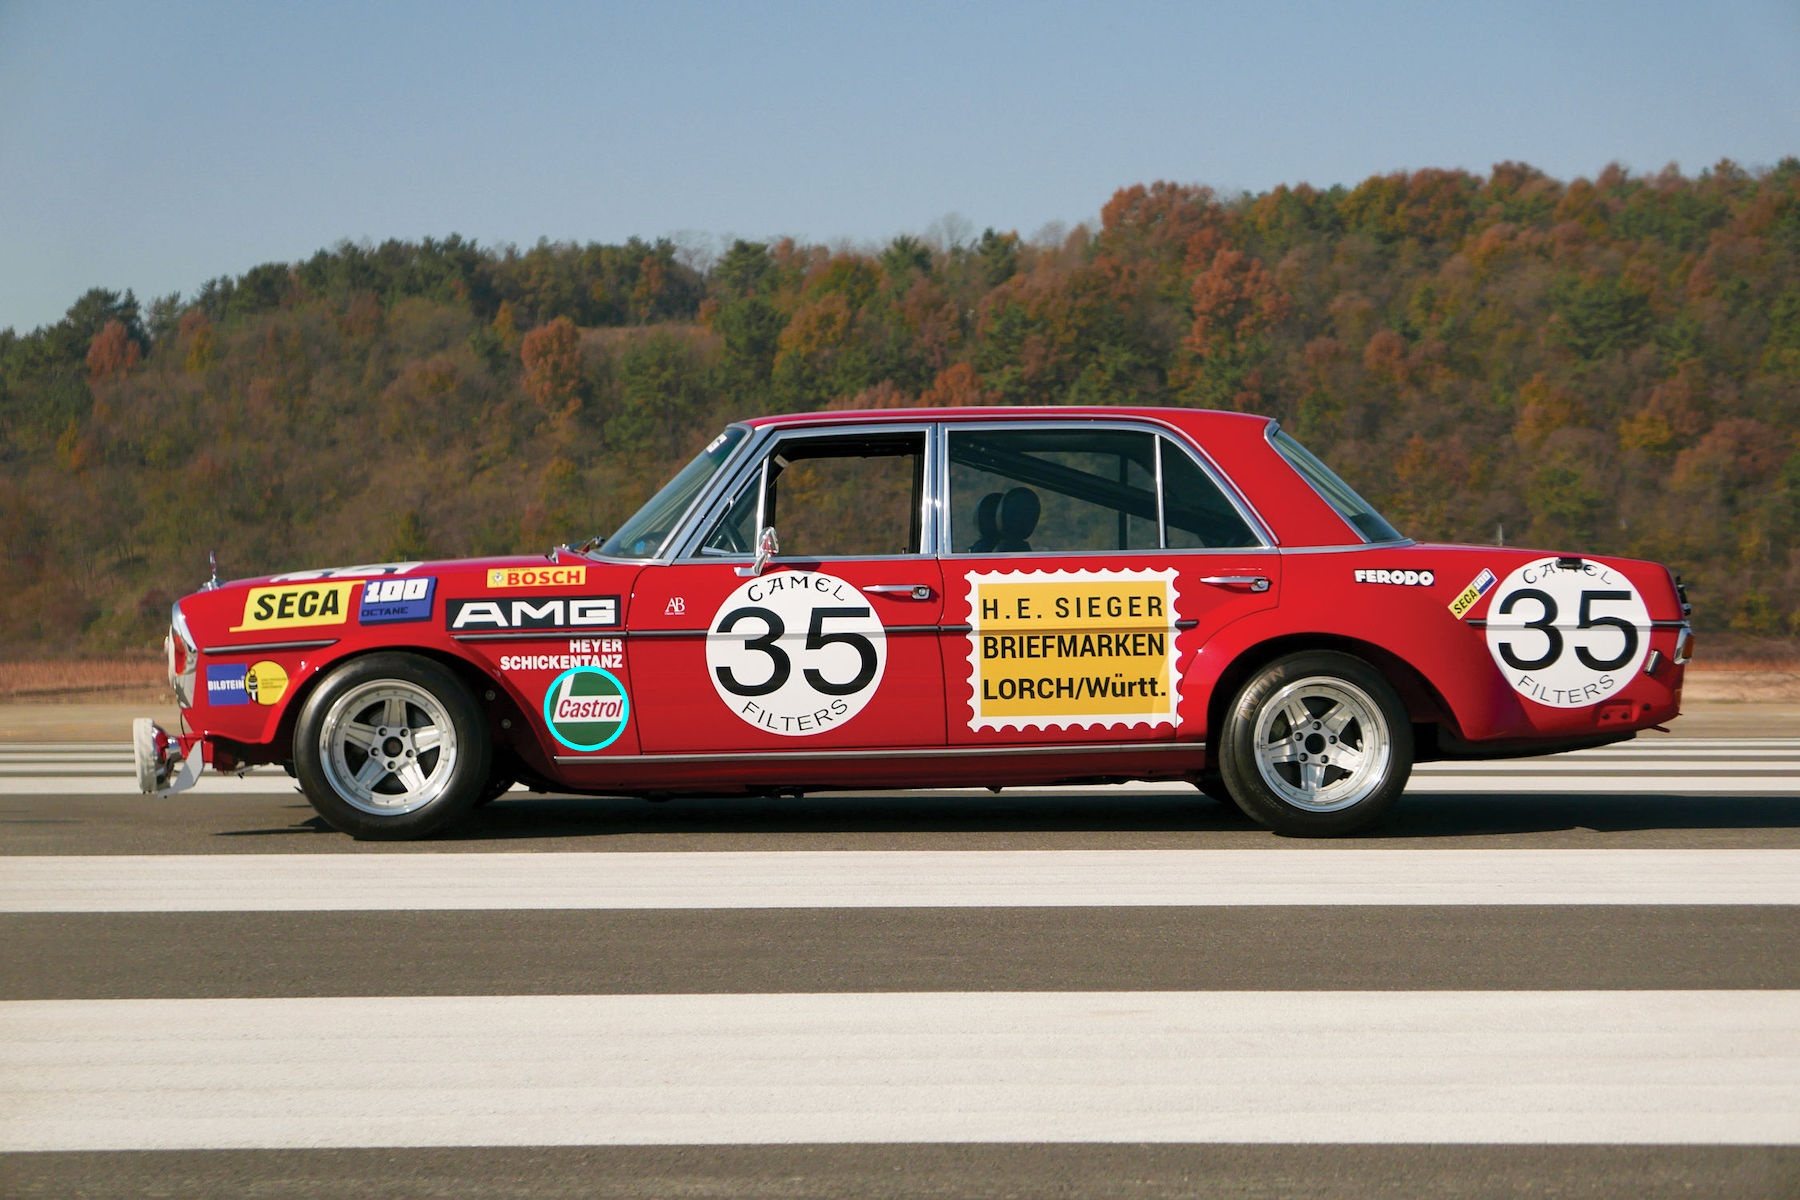
\includegraphics[width=\textwidth]{images/circles/Mercedes_SP.jpg}
        \caption{Результат преобразования Хафа для определенного радиуса окружностей}
        \label{img:mer_sp}
    \end{subfigure}
    \hfill
    \begin{subfigure}[b]{\textwidth}
        \centering
        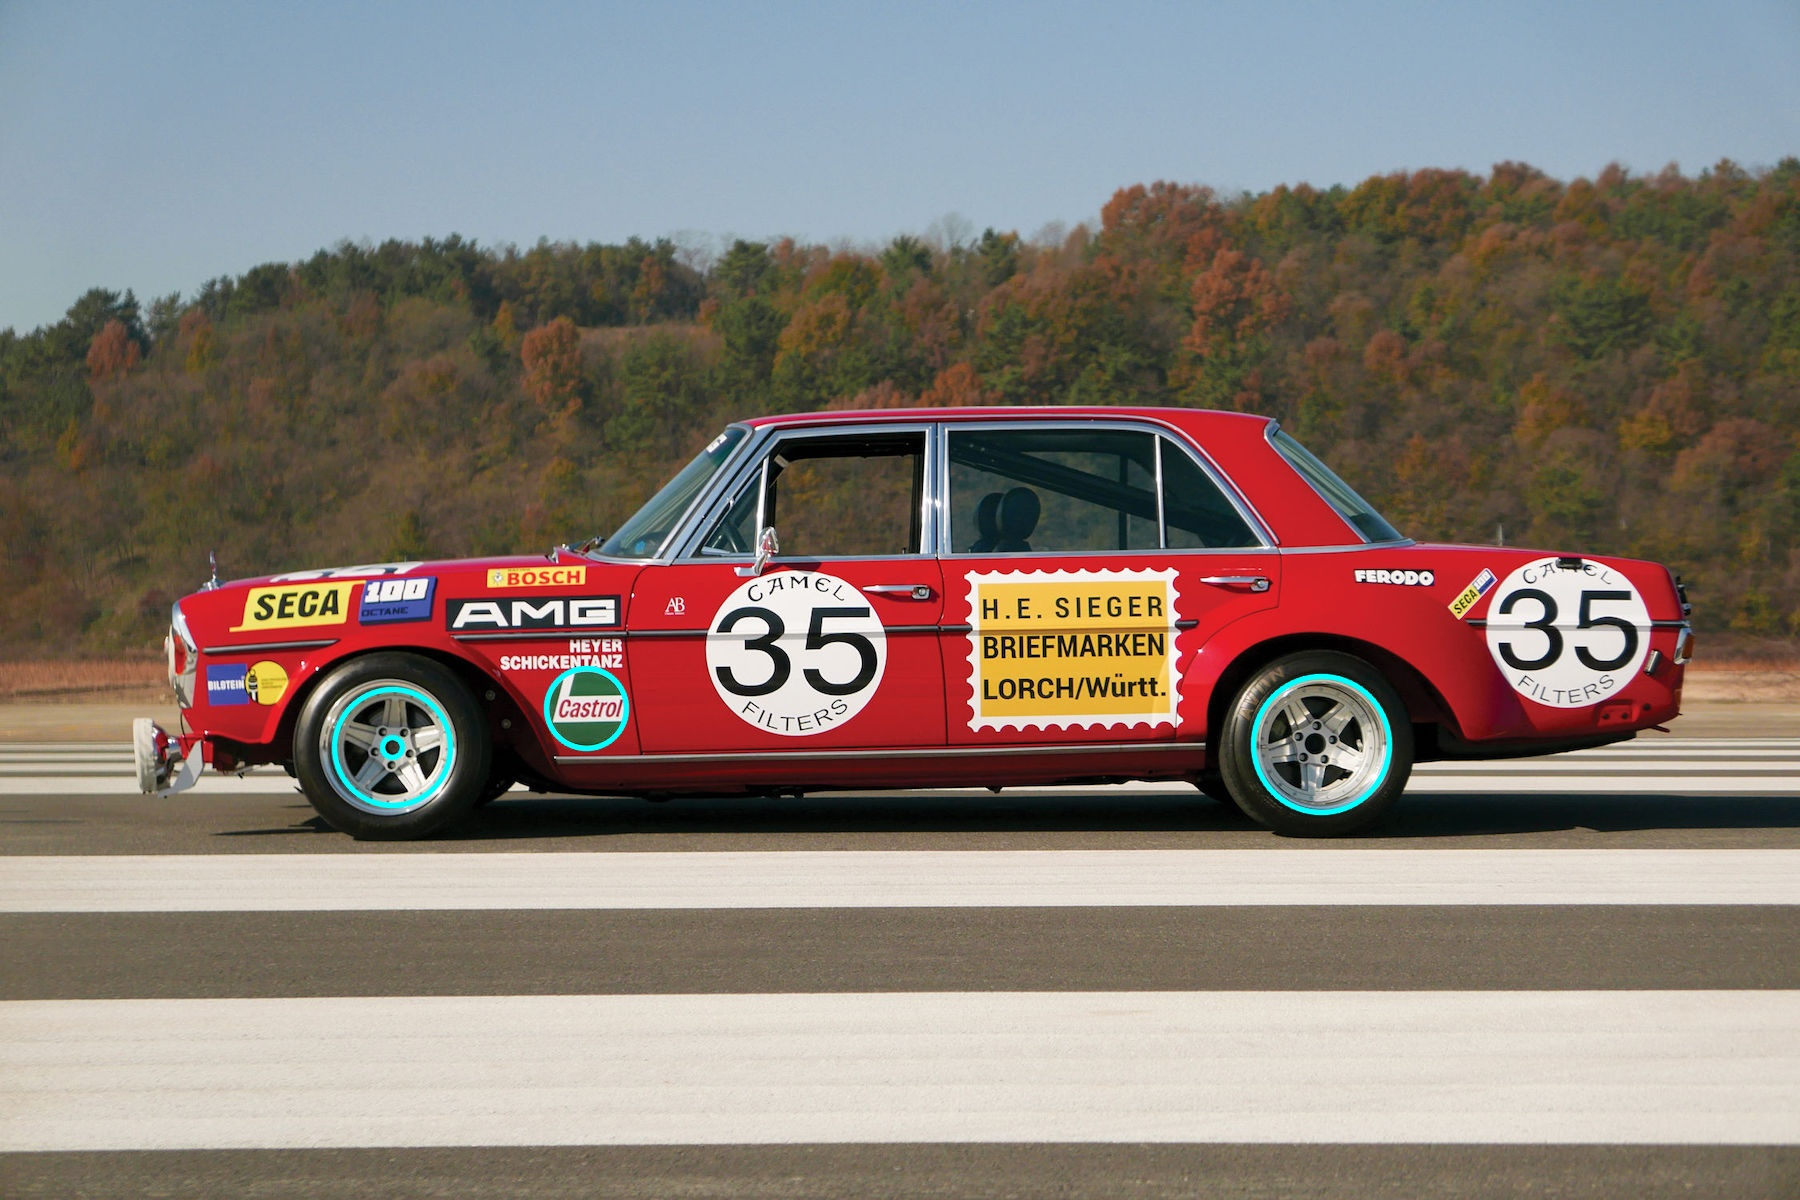
\includegraphics[width=\textwidth]{images/circles/Mercedes_R.jpg}
        \caption{Результат преобразования Хафа для диапазона радиусов}
        \label{img:mer_r}
    \end{subfigure}
        \caption{Результаты преобразования Хафа}
       \label{img::mer_comp}
\end{figure}

\clearpage

\section{Выводы}

В результате выполнения работы мы познакомились с преобразованием Хафа для поиска геометрических примитивов.

Стоит отметить, что важную роль в успешном определении прямых линий и окружностей играет оператор Кэнни, который обнаруживает контуры изображения. Нам удалось убедиться в этом при использовании полутонового изображения для преобразования Хафа: результаты при обнаружении прямых были удручающими (см. рисунки \ref*{img:fin_ITMO_gray}, \ref*{img:fin_fir_gray} и \ref*{img:fin_piet_gray}), а при определении окружностей программа не смогла ничего вывести.

Полный код программы и изображения можно найти на \href{https://github.com/NikBrat/ComputerVision_Lab5}{GitHub}.

\section{Ответы на вопросы}

\newcounter{question}
\setcounter{question}{0}

\newcommand{\question}[1]{\item[Q\refstepcounter{question}\thequestion.] #1}
\newcommand{\answer}[1]{\item[A\thequestion.] #1}


\begin{itemize}

    \question{Какая идея лежит в основе преобразования Хафа?}
   
    \answer{ В основе данного преобразования лежит идея поиска общего геометрического места точек (ГМТ) с помощью метода <<голосования>> точек. В классическом преобразовании также используется идея пространства параметров $(\theta, \rho)$ уранения прямой $y=kx+b$ $\Leftrightarrow$ $xcos(\theta)+ysin(\theta)=\rho$}
    
    \question{Можно ли использовать преобразование Хафа для поиска произвольных контуров, которые невозможно описать аналитически?}
    \answer{Решение данной задачи возможно при использовании \textbf{обобщеннго преобразования Хафа}.} 

    \question{Что такое рекуррентное и обобщенное преобразования Хафа?}
    \answer{Особенность рекуррентного преобразования Хафа заключается в том, что мы применяем преобразование в скользящем окне, определяя аккумулятор преобразования для каждой области, после чего будем составлять общий аккумуляторный массив. В результате каждая точка общего аккумулятора будет характеризоваться параметрами наиболее достоверного отрезка прямой, проходящего через него.
    
    Обобщенное преобразование Хафа применяется для случая произвольных контуров, не описываемых аналитически. В данном случае функция расстояния от пикселя границы до центра является функцией $R(\phi)$ от угла $\phi$ радиус-вектора, направленного от точки контура к центру(точка локализации). При этом $\phi$ может являться не только углом абсолютного направления на центр, но и относительным углом между направлением градиента и направлением радиуса-вектора.}

    \question{Какие бывают способы параметризации в преобразовании Хафа?}
    \answer{Бывают следующие способы параметризации: точки периметра $(n,m)$ сетки изображения, точка периметра и угол $(\alpha, n)$, Наклон и смещение $(\alpha, d)$, основание нормали.}
\end{itemize} % Content

% \include{source_codes_appendix}

\end{document}